%%%%%%%%%%%%%%%%%%%%%%%%%%%%%%%%%%%%%%%%%%%%%%%%%%%%%%%%%%%%%%%%%%%%%%%%%%%%%%%%%%%%%
%																					%
%	TRABAJO: Paper Mejoras en el procesador de Redes de Petri						%
%																					%
%		Titulo: 	Soft Core parametrizable con procesamiento de Redes de Petri	%
%																					%
%		Autores:	Julian Nonino													%
%					Carlos Renzo Pisetta											%
%					Orlando Micolini												%
%																					%
%	Seccion: ANALSIS DE RENDIMIENTO													%	
%	Archivo: analisis_rendimiento.tex												%
%																					%
%%%%%%%%%%%%%%%%%%%%%%%%%%%%%%%%%%%%%%%%%%%%%%%%%%%%%%%%%%%%%%%%%%%%%%%%%%%%%%%%%%%%%

 \section{An�lisis de Rendimiento}
 		Para comprobar  correcto funcionamiento del IP Core y analisar los tiempos de sincronizaci�n, se 
 		realizaron mediciones para distinto n�mero de iteraciones. Luego se compararo el Procesador de Petri 
 		con una implementaci�n utilizando sem�foros, ambos resolviendo un mismo problema. La elecci�n de este 
 		segundo m�todo de sincronizaci�n se basa en que son el mecanismo m�s ligero para realizar �stas tareas.
 		A partir de estas mediciones se realiz� la gr�fica de la Figura \ref{fig:resultados13} 
 		
		\begin{figure}[h]
			\centering
			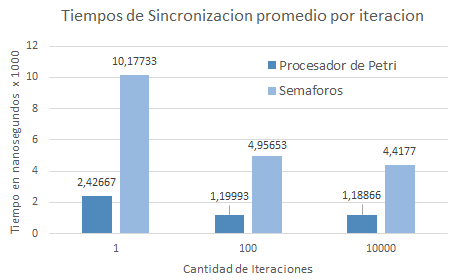
\includegraphics[width=3in]{resultados13}
			\caption{Tiempos de sincronizaci�n procesador de Redes de Petri vs. Sem�foros}
			\label{fig:resultados13}
		\end{figure}		
	
		Se puede observar que, para todos los casos, el procesador de Petri es aproximadamente cuatro veces
		m�s rapido que los Sem�foros.
		
		Esta medicion se realiz� con tiempos $\tau$ nulos, de manera que el rendimiento es el mismo obtenido
		en el procesador de Redes de Petri sin sem�ntica temporal. Esto es valido ya que el tiempo de una 
		transici�n es parte del modelo ,es decir, es el mismo para el procesador de petri como para la 
		implementeci�n con sem�foros. 
		
		Ademas como se observa en la  Figura \ref{fig:timed}, el procesador necesita �nicamente un 
		semi-ciclo de reloj, desde que el contador alcanza el valor $\tau$ hasta que el disparo se coloca
		en la cola de salida. La demora introducida es despreciable en relaci�n con
		el tiempo que tiene un $\Delta$T de un ciclo de reloj.	 
		
		\begin{figure}[h]
			\centering
			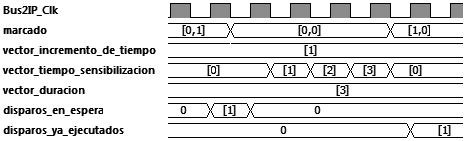
\includegraphics[width=3.5in]{timed}
			\caption{Tiempos de ejecuci�n2 }
			\label{fig:timed}
		\end{figure}

	Teniendo en cuenta la latencia despreciable y tomando el tiempo como parte del modelo
	es posible analizar el rendimiento sin tener en cuenta	el tiempo.
		
				
		
		 
		
		
		
		